

\documentclass{beamer}
\usepackage[utf8]{inputenc}
\usepackage[T1]{fontenc}

\usepackage{amsmath}
\usepackage{mathtools}
\usepackage{amsthm}
\usepackage{amssymb}
\usepackage{tcolorbox}
\tcbuselibrary{theorems}
\usepackage{tikz-cd}
\usepackage{xparse}
\usepackage{adjustbox}



\usepackage{tabularx}

%\newcommand{\cat}[1]{\mathcal{#1}}



\title{Hopf-Frobenius Modules and the Lie Correspondence}

\author{Matt Alexander}
\usetheme{queer}


%\newcommand{\newthought}[1]{\medskip\noindent\fbox{{#1}}}




%=================================
% Colourblind-friendly colours
%=================================


% 6 Colour Attempt Feb 27, 2024


\definecolor{lemmacolour}{RGB}{0, 0, 153} 


\definecolor{propcolour}{RGB}{138, 10,0}

\definecolor{definitioncolour}{RGB}{100, 100, 100}

\definecolor{examplecolour}{RGB}{62,217,141}

\definecolor{conjecturecolour}{RGB}{235, 160, 215}

\definecolor{theoremcolour}{RGB}{255, 240, 0}



%============================
% 5 Colour Attempt
%============================



%\definecolor{corolcolour}{RGB}{0, 114, 178}


%Compare this one and examplecolor on tritanopia
%\definecolor{lemmacolour}{RGB}{0, 114, 178} 
%
%
%\definecolor{propcolour}{rgb}{0.6, 0.0,0.0}
%
%
%\definecolor{theoremcolour}{rgb}{1.0, 0.84, 0.0}
%
%
%
%
%\definecolor{examplecolour}{RGB}{59,191,143}
%
%\definecolor{definitioncolour}{rgb}{0.75, 0.75, 0.75}



%============================
% Theorem Environments
%============================


\usepackage{}



\newenvironment{proof-lemma}
    {\begin{mdframed}[linewidth=3, linecolor=lemmacolour,topline=false,rightline=false,bottomline=false]
\begin{proof}
}{
\end{proof}
\end{mdframed}}


\newenvironment{proof-prop}
    {\begin{mdframed}[linewidth=3, linecolor=propcolour,topline=false,rightline=false,bottomline=false]
\begin{proof}
}{
\end{proof}
\end{mdframed}}


\newenvironment{proof-theorem}
    {\begin{mdframed}[linewidth=3, linecolor=theoremcolour,topline=false,rightline=false,bottomline=false]
\begin{proof}
}{
\end{proof}
\end{mdframed}}

\newenvironment{proof-corol}
    {\begin{mdframed}[linewidth=3, linecolor=lemmacolour,topline=false,rightline=false,bottomline=false]
\begin{proof}
}{
\end{proof}
\end{mdframed}}

\newenvironment{defframe}
    {\begin{mdframed}[linewidth=3, linecolor=definitioncolour,topline=false,rightline=false,bottomline=false]
}{
\end{mdframed}}

\newenvironment{exampleframe}
    {\begin{mdframed}[linewidth=3, linecolor=examplecolour,topline=false,rightline=false,bottomline=false]
}{
\end{mdframed}}

\newenvironment{conjecframe}
    {\begin{mdframed}[linewidth=3, linecolor=conjecturecolour,topline=false,rightline=false,bottomline=false]
}{
\end{mdframed}}



%============================

%\newtcbtheorem[number within=section]{theorem}{\color{black}Theorem}%
%{colback=theoremcolour!5,colframe=theoremcolour,fonttitle=\bfseries}{th}





%==========================================



%==============================================
% Theorems v.2
%==============================================


\newtcbtheorem[number within=section]{deff}{Definition}%
{colback=definitioncolour!5, colframe=definitioncolour,fonttitle=\bfseries}{th}


\newtcbtheorem[number within=section]{lemm}{Lemma}%
{colback=lemmacolour!5,colframe=lemmacolour!95!black,fonttitle=\bfseries}{th}



% Had to change this just for this presentation, so we didn't get prop 0.1, since there are no 'sections' in a beamer presentation.

\newtcbtheorem{prop}{Proposition}%
{colback=propcolour!5,colframe=propcolour,fonttitle=\bfseries}{th}



\newtcbtheorem[number within=section]{corol}{Corollary}%
{colback=corolcolour!5,colframe=corolcolour!95!black,fonttitle=\bfseries}{th}

\newtcbtheorem[number within=section]{exam}{Example}%
{colback=examplecolour!5,colframe=examplecolour,{fonttitle=\bfseries \color{black}}}{th}



\newtcbtheorem[number within=section]{conj}{Conjecture}%
{colback=conjecturecolour!5,colframe=conjecturecolour,{fonttitle=\bfseries \color{black}}}{th}


\newtcbtheorem[number within=section]{thm}{\color{black}Theorem}%
{colback=theoremcolour!5,colframe=theoremcolour,{fonttitle=\bfseries \color{black}},
label type=theorem}{thm}



%==============================================
% Theorems v.1
%==============================================


%\newtcbtheorem[number within=section]{definition}{Definition}%
%{colback=definitioncolour!5,colframe=definitioncolour!50!black,fonttitle=\bfseries}{th}
%
%
%\newtcbtheorem[number within=section]{lemma}{Lemma}%
%{colback=lemmacolour!5,colframe=lemmacolour!95!black,fonttitle=\bfseries}{th}
%
%
%\newtcbtheorem[number within=section]{prop}{Proposition}%
%{colback=propcolour!5,colframe=propcolour,fonttitle=\bfseries}{th}
%
%
%
%\newtcbtheorem[number within=section]{corollary}{Corollary}%
%{colback=corolcolour!5,colframe=corolcolour!95!black,fonttitle=\bfseries}{th}
%
%\newtcbtheorem[number within=section]{example}{Example}%
%{colback=examplecolour!5,colframe=examplecolour!90!black,fonttitle=\bfseries}{th}
%
%
%
%\newtcbtheorem[number within=section]{conjecture}{Conjecture}%
%{colback=conjecturecolour!5,colframe=conjecturecolour!90!black,fonttitle=\bfseries}{th}
%
%
%\newtcbtheorem[number within=section]{theorem}{\color{black}Theorem}%
%{colback=theoremcolour!5,colframe=theoremcolour,{fonttitle=\bfseries \color{black}},
%label type=theorem}{thm}








%\usepackage[demo]{graphicx}
\usepackage{wallpaper}
\usepackage{wrapfig,booktabs}

\usepackage{fancyhdr}
\usepackage{lettrine}

\usepackage{mdframed}

\usepackage{cancel}

%\usepackage{geometry}
%\geometry{
%tmargin=5cm, 
%bmargin=5cm, 
%lmargin=5cm, 
%rmargin=3cm,
%headheight=1.5cm,
%headsep=0.8cm,
%footskip=0.5cm}


\usepackage{tabularx}

\usepackage{braket}




%=====================
% MATH
%=====================

\usepackage{amsmath}
\usepackage{mathtools}
\usepackage{amsthm}
\usepackage{amssymb}
\usepackage{tcolorbox}
\tcbuselibrary{theorems}
\usepackage{tikz-cd}
\usepackage{xparse}

% To get a get a nice curvy arrow to talk about paths
\DeclareSymbolFont{lasy}{U}{lasy}{m}{n}
\SetSymbolFont{lasy}{bold}{U}{lasy}{b}{n}
\DeclareMathSymbol\leadsto{\mathrel}{lasy}{"3B}



% To have arrow heads in the middle
\usetikzlibrary{decorations.markings, arrows.meta}
\tikzset{
    marrow/.style={decoration={markings,mark=at position 0.5 with {\arrow{#1}}}, postaction=decorate}
}


%\usepackage[colorlinks=true]{hyperref}

\usepackage[nameinlink]{cleveref} % Better references to lemmas etc. The nameinlink makes all of 'Theorem 1' clickable


%\usepackage{titling} %Lets you have more than one title in a document
% But this won't work with ams articles, so I'll need to add it in separately for my own work and comment it out for research articles


\usepackage{adjustbox}



\usepackage[nointegrals]{wasysym}

\usepackage{fontawesome} % really cool fonts like morph and obj
\usepackage{tikz}



%========================
% COMMANDS
%========================


\newcommand{\Def}[1]{\textbf{\boldmath{#1}}}



%Field Theory
\newcommand{\exten}[2]{{#2}_{#1}}



\newcommand{\colim}{\operatorname{colim}}

\newcommand{\tabitem}{~~\llap{\textbullet}~~}

\newcommand{\newthought}[1]{\medskip\noindent\fbox{{#1}}}


\newcommand{\abs}[1]{| #1 |}

\newcommand{\cat}[1]{\mathcal{#1}}


\newcommand{\coker}{\operatorname{coker}}

\newcommand{\im}{\operatorname{Im}}

\newcommand{\const}{\text{\faAsterisk}}


\newcommand{\obj}{\text{\faCube}}

\newcommand{\morph}{\text{\faLocationArrow}}

\newcommand{\mor}[2]{\text{Mor}(#1, #2)}

\newcommand{\nbh}[1]{\mathcal{N}_{#1}} % The set of neighbourhoods around $x$.


\newcommand{\twist}{\text{\faRefresh}}


%================================
% HOMOTOPY / MODEL CATEGORIES
%=================================

\newcommand{\cyl}{\text{\faDatabase}}

\newcommand{\paths}{\text{\faPencilSquareO }}


%
%\newcommand{\bnbh}[1]{\mathcal{B}_{#1}}
%
%\newcommand{\base}[1]{\langle \cdot #1 \cdot \rangle}

\newcommand{\norm}[1]{\left\lVert #1 \right\rVert}

\newcommand{\gen}[1]{\left\langle #1 \right\rangle}

\newcommand{\triforce}{\resizebox{1em}{!}{
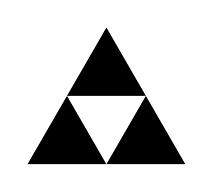
\begin{tikzpicture}
\fill[black] (0,0)  -- +(2,0) -- +(60:2) -- cycle;
\fill[white]  (60:1) -- +(1,0)  -- (1,0) -- cycle;
\end{tikzpicture}
}}





\begin{document}


\begin{frame}
\titlepage
\end{frame}


%===================
% SLIDE 1
%===================




%===================
% SLIDE 2
%===================


\begin{frame}

\frametitle{Definition of Frobenius Algebras}

%\framesubtitle{Part 3 --- Equivalences}

A Frobenius algebras is a unital associative $k$-algebra with a pairing $\gen{\cdot, \cdot}: F \otimes F \to k$, such that

\begin{itemize}
\item \newthought{Non-degenerate: } If $\gen{x,y} = 0$ for all $y$, then $x = 0$. Similarly, $\gen{x,y} = 0$ for all $x$ implies $y=0$.

\item \fbox{Associativity: } $\gen{xy,z} = \gen{x,yz}$, or in the complex case, $\gen{xy,z} = \gen{x, y^* z}$
\end{itemize}


\newthought{Equivalently: } A linear functional $\varepsilon: F \to k$, that satisfies the non-degeneracy condition
\begin{equation*}
\gen{x,y} = \varepsilon(xy) \quad \gen{x,y} = \varepsilon(x^* y)
\end{equation*}


\end{frame}


\begin{frame}

\frametitle{Definition of Frobenius Algebras}

\framesubtitle{Finite Dimensional Case}

An equivalent definition in the finite-dimensional case is a unital associative algebra, with maps $\Delta: F \to F \otimes F$, $\varepsilon: F \to k$ that satisfy 

\newthought{Coassociativity: } 
%
\begin{tikzcd}[ampersand replacement=\&]
F \ar[d, swap, "\Delta"] \ar[r, "\Delta"] \& F \otimes F \ar[d, "\Delta \otimes 1"] \\
F \otimes F \ar[r, "1 \otimes \Delta"] \& F \otimes F \otimes F
\end{tikzcd}


\newthought{Counitality: } 
%
\begin{tikzcd}[ampersand replacement=\&]
F \ar[d, swap, "\Delta"] \ar[r, "\Delta"] \ar[rrd, "1"] \& F \otimes F \ar[r, "\varepsilon \otimes 1"] \& k \otimes F \ar[d] \\
F \otimes F \ar[r, "1 \otimes \varepsilon"] \& F \otimes k \ar[r] \& F
\end{tikzcd}




\end{frame}


\begin{frame}

\frametitle{Definition of Frobenius Algebras}

\framesubtitle{Finite Dimensional Case}

\newthought{Frobenius Condition: } 

\begin{center}
\begin{tikzcd}[ampersand replacement=\&]
F \otimes F \ar[rr, "\Delta \otimes 1"] \ar[dd, "1 \otimes \Delta"] \ar[rd, "\mu"] \& \& F \otimes F \otimes F \ar[dd, "1 \otimes \mu"] \\
\& F \ar[rd, "\Delta"] \\
F \otimes F \otimes F \ar[rr, "\mu \otimes 1"] \& \& F \otimes F
\end{tikzcd}
\end{center}

\newthought{Sweedler Notation: } $\Delta: F \to F \otimes F$, so $x \in F$ is sent to $\Delta x = \sum_i a^i_x \otimes b^i_x$. We denote this by
\begin{equation*}
\Delta x = \sum x_{(1)} \otimes x_{(2)}
\end{equation*}




\end{frame}





\begin{frame}
\frametitle{Frobenius Algebras}

\framesubtitle{Examples}



\begin{tabularx}{\textwidth}{lll>{\raggedright\arraybackslash}X}
\toprule
Space & $\mu$ & $\gen{\cdot, \cdot}$ 
\\
\midrule
\\
$C_c^{\infty}(X)$ & Pointwise & $\gen{f,g} = \int f^* g$ \\
Schwartz functions $\cat{S}$ & Pointwise & $\gen{f,g} = \int f^* g$
\\
\\
$\mathbb{R}^n$ w/ basis $\{ e_i \}$ & $e_i e_j = \delta_{ij} e_i$ & $\gen{e_i,e_j} = \delta_{ij}$ \\
Hilbert space w/ basis $\{ e_i \}$ & $e_i e_j = \delta_{ij} e_i$ & $\gen{e_i,e_j} = \gen{e_i, e_j}_H$  \\
\\
$kG$ (finite group) & Group mult. & $\gen{g,h} = \delta_{gh, 1}$ 
\\
\bottomrule
\end{tabularx}

\medskip


\begin{equation*}
\cat{S} = \{ f \in C^{\infty}(\mathbb{R}^n, \mathbb{C}) \mid \sup_{x} \abs{x^\alpha D^\beta f(x)} < \infty, \forall \alpha, \beta \}
\end{equation*}



\end{frame}

%===================
% SLIDE 3
%===================


\begin{frame}
\frametitle{Hopf Algebras}

\framesubtitle{Definition}

A Hopf algebra is a unital associative $k$-algebra, $H$, with maps 

\medskip

\begin{itemize}
\item \fbox{Comultiplication: } $\Delta: H \to H \otimes H$

\item \fbox{Counit: } $\varepsilon: H \to k$

\item \fbox{Antipode: } An involution $S: H \to H$
\end{itemize}

\medskip

which satisfy the following:

\newthought{Coassociativity/Counitality: } 

\begin{tikzcd}[ampersand replacement=\&]
H \ar[d, swap, "\Delta"] \ar[r, "\Delta"] \& H \otimes H \ar[d, "\Delta \otimes 1"] \\
H \otimes H \ar[r, "1 \otimes \Delta"] \& H \otimes H \otimes H
\end{tikzcd}
%\quad
\begin{tikzcd}[ampersand replacement=\&]
H \ar[d, swap, "\Delta"] \ar[r, "\Delta"] \ar[rrd, "1"] \& H \otimes H \ar[r, "\varepsilon \otimes 1"] \& k \otimes H \ar[d, "\cong"] \\
H \otimes H \ar[r, "1 \otimes \varepsilon"] \& H \otimes k \ar[r, swap, "\cong"] \& H
\end{tikzcd}

\end{frame}



\begin{frame}
\frametitle{Hopf Algebras}

\framesubtitle{Definition}






\newthought{Bialgebra Condition: } $\Delta$ and $\varepsilon$ are algebra homomorphisms

\medskip

\newthought{Antipode Condition: } 

\begin{center}
\begin{tikzcd}[ampersand replacement=\&]
H \ar[rd, "\varepsilon"] \ar[r, "\Delta"] \ar[dd, swap, "\Delta"]  \& H \otimes H \ar[r, "S \otimes 1"] \& H \otimes H \ar[dd, "\mu"] \\
\& k \ar[rd, "\eta"] \\
H \otimes H \ar[r, "1 \otimes S"] \& H \otimes H \ar[r, "\mu"] \& H
\end{tikzcd}
\end{center}



\end{frame}







\begin{frame}


\frametitle{Hopf Algebras}
%

\framesubtitle{Examples}

\begin{tabularx}{\textwidth}{lll>{\raggedright\arraybackslash}X}
\toprule
Space & $\Delta$ & $\varepsilon$
\\
\midrule
\\
$kG$  & $\Delta g = g \otimes g$ & $\varepsilon(g) = 1$ \\
\\
Tensor alg. $T(X)$ & $\Delta x = x \otimes 1 + 1 \otimes x$ & $\varepsilon(x) = 0$ \\
Symmetric alg. $S(X)$ & $\Delta x = x \otimes 1 + 1 \otimes x$ & $\varepsilon(x) = 0$ \\
Univ. Env. Alg. $U(\mathfrak{g})$ & $\Delta x = x \otimes 1 + 1 \otimes x$ & $\varepsilon(x) = 0$
\\
\\
$\Lambda(X)$ & $\Delta x = x \otimes 1 - 1 \otimes x$ & $\varepsilon(x) = 0$
\\
\bottomrule
\end{tabularx}



\end{frame}

%===================
% SLIDE 4
%===================


\begin{frame}

\frametitle{Hopf-Frobenius Modules}
\framesubtitle{Definition}

A left Hopf-Frobenius module is a pair $(H,F)$ where $H$ is a Hopf algebra, $F$ is a Frobenius algebra and $F$ is a left $H$-module, such that the following conditions are satisfied:

\bigskip

\begin{itemize}


\item \fbox{Weak Cartan: }  $\sum \gen{g_{(1)} \cdot x, g_{(2)} \cdot y} = \varepsilon(g) \gen{x,y}$

\medskip

\item \fbox{Antipode Condition: }  $\gen{S(g) \cdot x, y} = \gen{x, g \cdot y}$

\end{itemize}





\end{frame}


\begin{frame}

\frametitle{Hopf-Frobenius Modules}
\framesubtitle{Example 1 --- Derivatives of Functions}


Take our Hopf algebra to be $k[\partial]$ and the Frobenius algebra to be $\cat{S}$, the space of Schwartz functions. This is an HF-module with

\bigskip

\begin{itemize}

\item \fbox{Action: } $\partial \cdot f = f'$, the derivative of $f$


\medskip

\item \fbox{Weak Cartan / Antipode: } Both of these conditions reduce to

\begin{equation*}
\int (\partial \cdot f) g  = - \int f (\partial \cdot g)
\end{equation*}
The \textbf{weak derivative} condition.
% $\gen{\partial f, g} + \gen{f, \partial g} = \varepsilon(\partial) \gen{f,g} = 0$. So
%\begin{equation}
%\int (\partial f) g + \int f (\partial g) = 0
%\end{equation}
%
%\item \fbox{Antipode: } $S(\partial) = - \partial$
\end{itemize}


\end{frame}



\begin{frame}

\frametitle{Hopf-Frobenius Modules}
\framesubtitle{Example 2 --- Operators on a Hilbert Space}

Let $F$ be a separable Hilbert space, and let $\{ A_i \}$ be a family of compact mutually-commuting \textit{skew-Hermitian} operators on $F$. Then we can find an orthonormal basis of simultaneous eigenvectors, $\{ e_k \}$. 

Take $(F, \{ e_k \})$ as our Frobenius algebra, and let $H = U(\{ A_i \} )$ be the universal enveloping algebra of the abelian Lie algebra generated by the $\{ A_i \}$. This is a HF-module where


\begin{itemize}

\item \fbox{Action: } $A_i \cdot e_k = A_i e_k = \alpha_{i}^k e_k$, the natural action of the Hermitian operators on the eigenvector basis.


\medskip

\item \fbox{Weak Cartan / Antipode: } Both of these conditions reduce to

\begin{equation*}
\gen{H x, y} = - \gen{x, Hy}
\end{equation*}
The \textbf{skew-Hermitian} condition.
\end{itemize}



\end{frame}





\begin{frame}

\frametitle{Hopf-Frobenius Modules}
\framesubtitle{Example 3 --- Lie Groups}


Consider the Lie group $O(n)$, and let $H$ be its group algebra over $\mathbb{R}$. Take $\mathbb{R}^n$ with basis $\{ e_i \}$ as our Frobenius algebra.

\bigskip

\begin{itemize}

\item \fbox{Action: } Left multiplication


\medskip

\item \fbox{Weak Cartan / Antipode: } Both of these conditions reduce to

\begin{equation*}
\gen{g \cdot x, g \cdot y} = \gen{x,y}
\end{equation*}
The orthogonality condition.

\end{itemize}




\end{frame}



\begin{frame}

\frametitle{Hopf-Frobenius Modules}
\framesubtitle{Example 3 --- Lie Groups}

\framesubtitle{Examples}

\begin{tabularx}{\textwidth}{lll>{\raggedright\arraybackslash}X}
\toprule
Group & Frobenius Algebra & $\gen{\cdot, \cdot}$ \\
\\
\midrule
\\
O(n) & $\mathbb{R}^n$ & Euclidean inner product \\
 U(n) & $\mathbb{C}^n$  & Complex inner product \\
 Sp(n) & $\mathbb{R}^{2n}$ & Symplectic inner product \\
\\
\bottomrule
\end{tabularx}





\end{frame}

\begin{frame}

\frametitle{Hopf-Frobenius Modules}
\framesubtitle{Example 4 --- Lie Algebras}


Consider the Lie algebra $\mathfrak{o}(n)$, viewed as a Lie algebra of matrices, and let $H$ be its universal enveloping algebra over $\mathbb{R}$. Take $\mathbb{R}^n$ with basis $\{ e_i \}$ as our Frobenius algebra.

\bigskip

\begin{itemize}

\item \fbox{Action: } Left multiplication


\medskip

\item \fbox{Weak Cartan / Antipode: } Both of these conditions reduce to

\begin{equation*}
\gen{A \cdot x, y} = - \gen{x,A \cdot y}, \quad A \in \mathfrak{o}(n)
\end{equation*}
The anti-symmetric condition.

\end{itemize}




\end{frame}








\begin{frame}

\frametitle{Weak Topology}

\framesubtitle{Frobenius Algebra}

Let $F$ be Frobenius. We consider the coarsest topology such that the maps
\begin{equation*}
\begin{split}
F \xrightarrow{\abs{\gen{x, -} }} k \\
F \xrightarrow{\abs{ \gen{-, y}} } k
\end{split}
\end{equation*}
are continuous for all $x,y \in F$, which we call the \textbf{weak topology} on $F$

\medskip

\newthought{Example: } The weak topologies on $\mathbb{R}^n$ and $\mathbb{C}^n$ are the standard topologies.

\end{frame}






\begin{frame}
\frametitle{Lie Algebra $\to$ Lie Group}

\framesubtitle{Example ---  $\mathfrak{o}(n)$}


Consider the HF-module of $H = U(\mathfrak{o}(n))$ acting on $\mathbb{R}^n$ with basis $\{ e_i \}$.

\bigskip

A general element of $\mathfrak{o}(3)$ is
\begin{equation*}
\begin{pmatrix}
0 & -a & -b \\
a & 0 & -c \\
b & c & 0
\end{pmatrix}
\end{equation*}

\newthought{Generators: } The action is generated by $p_{ij}$ with $p_{ij} e_i = e_j$, $p_{ij} e_j = - e_i$, $p_{ij} e_k = 0$, for $k \ne i,j$


\begin{equation*}
p_{12} = \begin{pmatrix}
0 & -1 & 0 \\
1 & 0 & 0 \\
0 & 0 & 0
\end{pmatrix}, \; p_{13} = \begin{pmatrix}
0 & 0 & -1 \\
0 & 0 & 0 \\
1 & 0 & 0
\end{pmatrix} \; p_{23} = \begin{pmatrix}
0 & 0 & 0 \\
0 & 0 & -1 \\
0 & 1 & 0
\end{pmatrix}
\end{equation*}




\end{frame}

%
%\begin{frame}
%
%%
%%$\gen{g x, gy} = \gen{x,y} + \beta (\gen{x, p_{ij} y} + \gen{p_{ij} x, y}) + (\gen{(1-\alpha) p_{ij}^2 x, y} + \gen{x, (1-\alpha) p_{ij}^2 y} ) + \beta^2 \gen{p_{ij} x, p_{ij} y} + \beta (\gen{(1-\alpha) p_{ij}^2 x, p_{ij} y} + \gen{p_{ij} x, (1-\alpha) p_{ij}^2 y} ) + (\gen{(1-\alpha) p_{ij}^2 x, (1-\alpha) p_{ij}^2 y} )$
%%
%%$= \gen{x,y} + \beta (\gen{x, p_{ij} y} + \gen{p_{ij} x, y}) + (2(1-\alpha) - \beta^2 - (1-\alpha)^2)(\gen{ x, p_{ij}^2 y}) +  \beta (1-\alpha) (\gen{ p_{ij}^2 x, p_{ij} y} + \gen{p_{ij} x, p_{ij}^2 y} )$
%%
%%
%%
%%%$= \gen{x,y} + \beta (\gen{x, p_{ij} y} + \gen{p_{ij} x, y}) + ((1-\alpha)(1+\alpha) - \beta^2)(\gen{ x, p_{ij}^2 y}) +  \beta (1-\alpha) (\gen{ p_{ij}^2 x, p_{ij} y} + \gen{p_{ij} x, p_{ij}^2 y} )$
%
%
%
%
%\end{frame}




\begin{frame}

\frametitle{Lie Algebra $\to$ Lie Group}

\framesubtitle{Example ---  $\mathfrak{o}(n)$}

\newthought{Annihilator: } Let $\operatorname{ann} F = \{ g \in H \mid g x = 0$ for all $x \in F \}$. Consider the quotient
%
\begin{equation*}
H/\operatorname{ann} F
\end{equation*}

\newthought{Grouplike elements: } Let $g_{ij} = 1 + \beta \bar{p}_{ij} + (1 - \alpha) \bar{p}_{ij}^2$ in $H/ \operatorname{ann} F$

\begin{equation*}
\begin{split}
\gen{g_{ij} x, g_{ij} y} = &\gen{x,y} \\
&+ \beta (\gen{x, \bar{p}_{ij} y} + \gen{\bar{p}_{ij} x, y})\\
&+ (1- (\alpha^2 + \beta^2))(\gen{ x, \bar{p}_{ij}^2 y})\\
&+ \beta (1-\alpha) (\gen{ \bar{p}_{ij}^2 x, \bar{p}_{ij} y} + \gen{\bar{p}_{ij} x, \bar{p}_{ij}^2 y} )
\end{split}
\end{equation*}
for $\alpha^2 + \beta^2 = 1$, $g_{ij}$ behaves like a grouplike element in $H/\operatorname{ann} F$

\end{frame}


\begin{frame}

\frametitle{Lie Algebra $\to$ Lie Group}

\framesubtitle{Example ---  $\mathfrak{o}(n)$}



\newthought{Corresponding group: } We can show the following is a group

\begin{equation*}
\begin{split}
\operatorname{Gr}_F^H \equiv \{ g \in H/\operatorname{ann} F \mid &\gen{g x, gy} = \gen{S(g) x, S(g) y} = \gen{x,y} \\
&\text{ and } \gen{S(g) x, y} = \gen{x, gy} \}
\end{split}
\end{equation*}

\medskip

$\operatorname{Gr}^{U(\mathfrak{o}(n))}_{\mathbb{R}^n}$ is generated by the $g_{ij}$. Furthermore,
\begin{equation*}
\operatorname{Gr}^{U(\mathfrak{o}(n))}_{\mathbb{R}^n} \cong SO(n)
\end{equation*}
as a discrete group. But we get more!

\end{frame}





\begin{frame}

\frametitle{Lie Algebra $\to$ Lie Group}

\framesubtitle{Example ---  $\mathfrak{o}(n)$}






\newthought{Topology: } It also inherits the \textbf{appropriate topology} from $F$: the weak topology induced by the maps
\begin{equation*}
k \operatorname{Gr}^{U(\mathfrak{o}(n))}_{\mathbb{R}^n} \xrightarrow{ev_x} F
\end{equation*}
induces a topology on $\operatorname{Gr}^{U(\mathfrak{o}(n))}_{\mathbb{R}^n}$ which matches the standard topology $SO(n)$
\begin{equation*}
\operatorname{Gr}^{U(\mathfrak{o}(n))}_{\mathbb{R}^n} \cong SO(n)
\end{equation*}
as topological groups.

\end{frame}

%\begin{frame}
%\frametitle{Topology of Group}
%
%
%\end{frame}
%
%\begin{frame}
%\frametitle{Topology of Group: Left and Right Mult}
%
%
%\end{frame}
%
%\begin{frame}
%\frametitle{Topology of Group: Hausdorff}
%
%
%\end{frame}
%
%
%\begin{frame}
%\frametitle{Topology of Group: Locally Compact}
%
%
%\end{frame}
%
%\begin{frame}
%\frametitle{Topology of Group Matches}
%
%
%\end{frame}



\begin{frame}
\frametitle{Pathway for all Classical Lie Groups}


\begin{prop*}{}
Given any classical Lie algebra, $\mathfrak{g}$, with Lie group $G(\mathfrak{g})$ there is a Frobenius algebra $F_{\mathfrak{g}}$ such that $(U(\mathfrak{g}), F_{\mathfrak{g}})$ is a Hopf-Frobenius module, and 
\begin{equation*}
\operatorname{Gr}_{\mathfrak{g}}^{U(\mathfrak{g})} \cong G(\mathfrak{g})
\end{equation*}
as topological groups
\end{prop*}

\newthought{Lie Structure: } Every topological group has at most one Lie group structure, up to isomorphism.


\end{frame}



\begin{frame}
\frametitle{Lie Group $\to$ Lie Algebra: $O(n)$}

\begin{lemma}{}
Every antisymmetric matrix can be written as a linear combination of $O_i - O_i^T$ for some orthogonal matrices $O_i$
\end{lemma}


\newthought{Example: } 



\begin{equation*}
\sqrt{2} \begin{pmatrix}
0 & -1 & 0 \\
1 & 0 & 0 \\
0 & 0 & 0
\end{pmatrix} = \dfrac{1}{\sqrt{2}} \begin{pmatrix}
1 & -1 & 0 \\
1 & 1 & 0 \\
0 & 0 & 1
\end{pmatrix} - \dfrac{1}{\sqrt{2}} \begin{pmatrix}
1 & 1 & 0 \\
-1 & 1 & 0 \\
0 & 0 & 1
\end{pmatrix}
\end{equation*}





%\newthought{Example: } Recall $g_{ij} = 1 + \beta \bar{p}_{ij} + (1-\alpha)^2 \bar{p}_{ij}^2$. Set 
%
% $p_{ij} = g_{ij} - g_{ij}^T$


\end{frame}


\begin{frame}
\frametitle{Lie Group $\to$ Lie Algebra}

Given any Hopf algebra $H$, the subspace
\begin{equation*}
\mathfrak{L}(H) = \operatorname{span}\{ x - S(x) \mid x \in H \}
\end{equation*}
has the structure of a Lie algebra under the commutator bracket.


\begin{prop*}{}{}
If $G$ is a classical Lie group with Lie algebra $\mathfrak{g}$,
\begin{equation*}
\mathfrak{L}(kG) \cong \mathfrak{g}
\end{equation*}
as Lie algebras.
\end{prop*}


\end{frame}



\begin{frame}

\frametitle{Lie Group $\rightleftarrows$ Lie Algebra}

We have a pair of constructions
\begin{equation*}
\operatorname{Gr}_F: \mathfrak{g} \rightleftarrows G : \mathfrak{L}
\end{equation*}
which reproduce the Lie correspondence on classical Lie groups/algebras

\bigskip

\newthought{Ado's theorem: } Every finite dimensional Lie algebra over a field of $\operatorname{char} = 0$ is isomorphic to some Lie algebra of square matrices with the commutator.


\end{frame}




\begin{frame}
\frametitle{Future Work}

\framesubtitle{Lie's Third Theorem}

\newthought{Non-classical Lie Algebras: } Lie's third theorem (every finite-dimensional Lie algebra comes from a Lie group) has notoriously deep proofs.\footnote{Mathoverflow has a nice discussion under, `Why is Lie's Third Theorem difficult?'} 

\medskip

Most proofs (for example those using Ado's theorem) aren't constructive

\bigskip

\newthought{Question: } Is there a (constructive?) proof of the theorem from the perspective of HF-modules?

\newthought{Goal: } Construct an appropriate Frobenius algebra, given a Lie algebra $\mathfrak{g}$


\end{frame}



\begin{frame}
\frametitle{Future Work}

\framesubtitle{Infinite Dimensional Lie Algebras}


Consider the algebra of Laurent polynomials, $\mathbb{C}[z, z^{-1}]$. Derivations on the algebra form a Lie algebra $\mathfrak{g}$ with basis $\{ z^n \partial \}$.

\medskip

$\mathfrak{g}$ acts on $\mathbb{C}[z, z^{-1}]$, but what is the Frobenius structure?


\medskip

\begin{equation*}
\varepsilon(p(z)) = \dfrac{1}{2 \pi i} \oint_{\gamma} p(z) dz = \operatorname{Res}(p(z), 0)
\end{equation*}
This is the only Frobenius structure which satisfies
\begin{equation*}
\gen{\partial p(z), q(z)} = - \gen{p(z), \partial q(z)}
\end{equation*}
But $\gen{z^n \partial p(z), q(z)} \ne - \gen{p(z), z^n \partial q(z)}$ for $n \ne 0$




\end{frame}


%
%
%
%\begin{frame}
%\frametitle{Lie Group $\to$ Lie Algebra}
%
%We can apply the construction $\mathfrak{L}$ to discrete groups
%
%
%\newthought{Example: } $Q_8$
%
%\end{frame}
%
%
%\begin{frame}
%
%
%$[\phi_{123}, \phi_{234}] = \phi_{143} - \phi_{124}$
%
%$[\phi_{123}, \phi_{124}] = \phi_{234} - \phi_{143}$
%
%$[\phi_{123}, \phi_{134}] = \phi_{124} - \phi_{234}$
%
%$[\phi_{234}, \phi_{124}] = \phi_{123} - \phi_{134}$
%
%$[\phi_{234}, \phi_{134}] = \phi_{142} - \phi_{123}$
%
%$[\phi_{124}, \phi_{134}] = \phi_{123} - \phi_{243}$
%
%
%\begin{itemize}
%
%\item
%
%$[\phi_{123}, \phi_{234}] = \phi_{143} - \phi_{124}$
%
%$[\phi_{234}, \phi_{341}] = \phi_{214} - \phi_{231}$
%
%$[\phi_{312}, \phi_{124}] = \phi_{342} - \phi_{314}$
%
%
%
%
%\item
%
%
%
%$[\phi_{124}, \phi_{134}] = \phi_{123} - \phi_{243}$
%
%
%
%\item
%
%$[\phi_{123}, \phi_{341}] = \phi_{124} - \phi_{234}$
%
%
%\item
%
%$[\phi_{342}, \phi_{241}] = \phi_{123} - \phi_{134}$
%
%
%\end{itemize}
%
%
%
%
%
%
%
%
%\end{frame}
%
%
%
%\begin{frame}
%\frametitle{Lie Algebra $\mathfrak{L}(A_n)$}
%
%
%if we have transpositions, they won't show up since they have order $2$
%
%$(ab)(bc) = (acb)$
%
%$A_n$ is generated by $3$-cycles
%
%$(Abc)(Ayz) = (Abcyz)$
%
%$(Abc)(xAz) = (Abczx)$
%
%$(Abc)(xyA)$ 5 cycle
%
%just cyclically permute
%
%2 in common
%
%$(ABc)(ABz) = (Az)(Bc)$
%
%$(ABc)(AyB) = (Bcy)$
%
%3 in common
%
%$(ABC)(ABC) = (ACB)$
%
%$(ABC)(CAB) = 1$
%
%
%
%
%
%
%\end{frame}
%
%
%\begin{frame}
%
%Let $\phi_g = g - g^{-1}$
%
%
%\begin{equation}
%\phi_{g} = - \phi_{g^{-1}}
%\end{equation}
%
%
%\begin{equation}
%[\phi_g, \phi_h] = \phi_{gh} - \phi_{hg} + \phi_{g h^{-1}} - \phi_{h^{-1} g}
%\end{equation}
%
%$(xyz)^{-1} = (xzy)$
%
%\begin{equation}
%[\phi_{(Abc)}, \phi_{(Ayz)}] = \phi_{(Abcyz)} - \phi_{(Ayzbc)} + \phi_{(Abczy)} - \phi_{(Azybc)}
%\end{equation}
%
%
%$\phi_{(ab)(cd)} = 0$ since it has order $2$
%
%
%swaps the last two digits
%
%
%\begin{equation}
%[\phi_{(ABc)}, \phi_{(ABz)}] = \phi_{(Az)(Bc)} - \phi_{(Ac)(Bz)} + \phi_{(Bcz)} - \phi_{(Azc)}
%\end{equation}
%
%$(AzB)(ABc) = (BAz)(BcA) = (Azc)$
%
%
%
%\end{frame}
%
%
%\begin{frame}
%
%
%\begin{equation}
%\begin{split}
%&[\phi_{(Abc)}, \phi_{(Ayz)}] = \phi_{(Abcyz)} - \phi_{(Ayzbc)} + \phi_{(Abczy)} - \phi_{(Azybc)} \\
%&[\phi_{(ABc)}, \phi_{(ABz)}] = \phi_{(Bcz)} - \phi_{(Azc)}
%\end{split}
%\end{equation}
%
%$[\phi_{(ABc)}, \phi_{(AyB)}] = [\phi_{(ABc)}, -\phi_{(ABy)}] = [\phi_{(ABy)}, \phi_{(ABc)}] = \phi_{(Byc)} - \phi_{(Acy)}$
%
%
%
%\end{frame}
%
%
%
%
%
%\begin{frame}
%
%\frametitle{$A_5$}
%
%subalgebra generated by the $3$-cycles
%
%$[\phi_{(ABc)}, \phi_{(ABz)}] = \phi_{(Bcz)} - \phi_{(Azc)} = \phi_{(Bcz)} + \phi_{(Acz)}$
%
%\begin{equation*}
%[\phi_{(ABc)}, \phi_{(ABz)}] = \phi_{(Acz)} + \phi_{(Bcz)}
%\end{equation*}
%
%
%\newthought{$A_4$: } $\{ \phi_{(123)}, \phi_{(124)}, \phi_{(134)}, \phi_{(234)} \}$
%
%\begin{equation}
%\begin{split}
%[\phi_{(123)}, \phi_{(124)}] &= \phi_{(134)} + \phi_{(234)} \\
%[\phi_{(132)}, \phi_{(134)}] &= \phi_{(124)} + \phi_{(324)} \\
%[\phi_{(142)}, \phi_{(143)}] &= \phi_{(123)} + \phi_{(423)} \\
%[\phi_{(234)}, \phi_{(231)}] &= \phi_{(241)} + \phi_{(341)} \\
%[\phi_{(124)}, \phi_{(234)}] &= - (\phi_{(213)} + \phi_{(413)}) \\
%[\phi_{(134)}, \phi_{(234)}] &= \phi_{(312)} + \phi_{(412)}
%\end{split}
%\end{equation}
%
%
%\end{frame}
%
%
%\begin{frame}
%
%
%\begin{equation}
%\begin{split}
%[\phi_{(123)}, \phi_{(124)}] &= \phi_{(134)} + \phi_{(234)} \\
%[\phi_{(123)}, \phi_{(134)}] &= \phi_{(234)} - \phi_{(124)} \\
%[\phi_{(124)}, \phi_{(134)}] &= \phi_{(123)} + \phi_{(234)} \\
%[\phi_{(234)}, \phi_{(123)}] &= \phi_{(124)} + \phi_{(134)} \\
%[\phi_{(124)}, \phi_{(234)}] &= \phi_{(123)} - \phi_{(134)} \\
%[\phi_{(134)}, \phi_{(234)}] &= \phi_{(123)} + \phi_{(124)}
%\end{split}
%\end{equation}
%
%
%%$[\phi_{123}, \phi_{234}] = \phi_{143} - \phi_{124}$
%%$[\phi_{123}, \phi_{124}] = \phi_{234} - \phi_{143}$
%%$[\phi_{123}, \phi_{134}] = \phi_{124} - \phi_{234}$
%%
%%$[\phi_{234}, \phi_{124}] = \phi_{123} - \phi_{134}$
%%
%%$[\phi_{234}, \phi_{134}] = \phi_{142} - \phi_{123}$
%%$[\phi_{124}, \phi_{134}] = \phi_{123} - \phi_{243}$
%
%
%\newthought{Maximal ideal: } $I = \{ \phi_{(123)} - \phi_{(134)}, \phi_{(134)} + \phi_{(234)}, \phi_{(234)} - \phi_{(124)} \}$
%
%You can check that $I$ is simple and $I \cong \mathfrak{su}(2)$. So
%\begin{equation}
%\mathfrak{L}(A_4) \cong \mathfrak{g}_1 \oplus \mathfrak{su}(2)
%\end{equation}
%where $\mathfrak{g}_1$ is the one-dimensional Lie algebra.
%
%\end{frame}
%
%
%\begin{frame}
%
%$[a,b] = c$
%
%$[b,c] = 8a$
%
%$[a,c] = -8b$
%
%This is isomorphic to $\mathfrak{su}(2) \cong \mathfrak{so}(3, \mathbb{R})$ as a Lie algebra over $\mathbb{R}$
%
%\begin{equation}
%\mathfrak{L}(A_4) \cong 
%\end{equation}
%
%%We'll try to show this is isomorphic to 
%%
%%$[x,y] = z$
%%$[y,z] = x$
%%$[x,z] = -y$
%
%$\phi([x,y]) = \phi(z) = [\phi(x), \phi(y)]$
%
%let $\phi(x) = \alpha_x a + \beta_x b + \gamma_x c$
%
%%$[\phi(x), \phi(y)] = \alpha_x \beta_y c + \alpha_x \gamma_y (-8b) + \beta_x \alpha_y (-c) + \beta_x \gamma_y (8a) + \gamma_x \alpha_y (8b) + \gamma_x \beta_y (-8a)$
%
%
%
%$[\phi(i), \phi(j)] = \alpha_i \beta_j c + \alpha_i \gamma_j (-8b) + \beta_i \alpha_j (-c) + \beta_i \gamma_j (8a) + \gamma_i \alpha_j (8b) + \gamma_i \beta_j (-8a)$
%
%\begin{equation}
%[\phi(i), \phi(j)] = 8(\beta_i \gamma_j - \gamma_i \beta_j) a + 8(\gamma_i \alpha_j - \alpha_i \gamma_j) b + (\alpha_i \beta_j -\beta_i \alpha_j ) c
%\end{equation}
%
%
%
%
%\end{frame}
%
%\begin{frame}
%adjoint representation
%
%
%\begin{equation}
%a = \begin{pmatrix}
%0 & 0 & 0 \\
%0 & 0 & -8 \\
%0 & 1 & 0
%\end{pmatrix} \; b = \begin{pmatrix}
%0 & 0 & 8 \\
%0 & 0 & 0 \\
%-1 & 0 & 0
%\end{pmatrix} \;
%c = \begin{pmatrix}
%0 & -8 & 0 \\
%8 & 0 & 0 \\
%0 & 0 & 0
%\end{pmatrix}
%\end{equation}
%
%
%use killing form
%\begin{equation}
%B = \begin{pmatrix}
%-16 & 0 & 0 \\
%0 & -16 & 0 \\
%0 & 0 & -128
%\end{pmatrix}
%\end{equation}
%
%all of the adjoint reps are diagonalizable, so the cartan subalgebra will just be one-dimensional (but they're only diagonalizable over $\mathbb{C}$, so that won't be enough for the real case)
%
%
%instead we look at a regular element
%
%the characteristic polynomials show us that our lie group has rank $1$. $a,b,c$ are all regular elements
%
%Then we get that our cartan subalgebra is just the one-dimensional $\gen{a}$. This is not a splitting subalgebra, since we can't get all of the eigenvalues of $a$
%
%\end{frame}
%
%
%
%
%\begin{frame}
%
%Now we find the casimir element
%
%the dual basis has $a^* = (-1/16) a$
%
%$a a^* + b b^* + c c^* = \dfrac{-1}{16} (a^2 + b^2) + \dfrac{-1}{128} c^2$
%
%
%
%\end{frame}
%
%
%\begin{frame}
%we end up with the equations
%
%$\alpha_x = 8(\beta_y \gamma_z - \gamma_y \beta_z)$
%$\beta_x = 8(\gamma_y \alpha_z - \alpha_y \gamma_z)$
%$\gamma_x = (\alpha_y \beta_z - \beta_y \alpha_z )$
%
%
%$\alpha_y = 8(\beta_z \gamma_x - \gamma_z \beta_x)$
%$\beta_y = 8(\gamma_z \alpha_x - \alpha_z \gamma_x)$
%$\gamma_y = (\alpha_z \beta_x - \beta_z \alpha_x )$
%
%$\alpha_z = 8(\beta_x \gamma_y - \gamma_x \beta_y)$
%$\beta_z = 8(\gamma_x \alpha_y - \alpha_x \gamma_y)$
%$\gamma_z = (\alpha_x \beta_y - \beta_x \alpha_y )$
%
%
%$\alpha_x = 8(\beta_y (\alpha_x \beta_y - \beta_x \alpha_y) - (\alpha_z \beta_x - \beta_z \alpha_x ) \beta_z)$
%
%\end{frame}
%
%
%
%
%\begin{frame}
%\frametitle{Lie Group $\to$ Lie Algebra}
%
%We can apply this construction to discrete groups as well
%
%
%\newthought{Example: } $S_4$
%
%
%$(123) - (213)$
%$(234) - (324)$
%$(124) - (214)$
%$(134) - (314)$
%
%8 terms
%
%$(1234) - (1432)$
%$(1243)$
%$(1342)$
%$(1324)$
%$(1423)$
%$(1432)$
%
%6 terms
%
%i think this gives the $g_2$ exceptional lie algebra
%
%
%$[g - S(g), h - S(h)] = [g,h] + [S(g), S(h)] - [g, S(h)] - [S(g), h] = [g,h] - S([g,h]) + [h,S(g)] - S([h,S(g)])$
%
%$= gh - S(gh) - (hg - S(hg)) + (g S(h) - S(gS(h)) ) - (S(h)g - S(S(h)g))$
%
%
%So $[\phi_g, \phi_h] = \phi_{gh} + \phi_{g^{-1} h^{-1}} + \phi_{g h^{-1}} + \phi_{g^{-1} h}$
%
%$[\phi_g, \phi_h] = \phi_{gh} - \phi_{hg} + \phi_{g h^{-1}} - \phi_{h^{-1} g}$
%
%$(123)(234) = (13)(24)$
%
%$(234)(123) = (12)(34)$
%
%if $xyxy = 1$ then $yxyxy = y$, so $yxyx = 1$. So as soon as we know one product has order 2, the opposite order does as well
%
%$(123)(324) = (143)$
%
%$(324)(123) = (124)$
%
%$[\phi_{123}, \phi_{234}] = 0 - 0 + \phi_{143} - \phi_{124}$
%
%
%
%[4] = 123
%%[3] = 132
%[12] = 234
%%[8] = 243
%[19] = 134
%%[11] = 143
%[20] = 124
%%[15] = 142
%
%$[\phi_{123}, \phi_{234}] = \phi_{143} - \phi_{124}$
%$[\phi_{123}, \phi_{124}] = \phi_{234} - \phi_{143}$
%$[\phi_{123}, \phi_{134}] = \phi_{124} - \phi_{234}$
%
%$[\phi_{234}, \phi_{124}] = \phi_{123} - \phi_{134}$
%
%$[\phi_{234}, \phi_{134}] = \phi_{142} - \phi_{123}$
%$[\phi_{124}, \phi_{134}] = \phi_{123} - \phi_{243}$
%
%[4][8] = [11]
%[4][15] = [12]
%[4][19] = [20]
%
%%[3][8] = 0
%%[3][11] = [8]
%%[3][12] = [15]
%%[3][15] = 0
%%[3][19] = 0
%%[3][20] = [19]
%
%[8][4] = [20]
%[8][11] = 0
%[8][15] = [11]
%[8][19] = [3]
%[8][20] = 0
%
%[11][3] = [15]
%[11][12] = [4]
%[11][20] = [8]
%
%[12][3] = [19]
%[12][11] = [15]
%[12][20] = [4]
%
%[15][4] = [11]
%[15][8] = [3]
%[15][19] = [12]
%
%[19][4] = [12]
%[19][8] = [20]
%[19][15] = [3]
%
%[20][3] = [8]
%[20][11] = [4]
%[20][12] = [19]
%
%
%
%\end{frame}
%
%
%%
%%
%
%%
%%
%%
%%%
%%\begin{tikzcd}[ampersand replacement=\&]
%%A \arrow[r, ""{name=U, below}] 
%%\& B \\
%%C \arrow[r, ""{name=D}]
%%\& D \arrow[Rightarrow, from=U, to=D]
%%\end{tikzcd}
%%
%
%
%%===================
%% SLIDE 4
%%===================
%%
%%
%%\begin{frame}
%%\frametitle{Definition of Genres}
%%\framesubtitle{Part 1 --- Morphisms}
%%
%%\begin{itemize}
%%\item \fbox{$n$-Morphisms: } For all $n \geq 0$ we have a set of $n$-morphisms, $G_n$
%%
%%\smallskip
%%
%%\item \fbox{Source/Target: } Every $n$-map has the shape $\phi: f \to g$, for $f, g \in G_{n-1}$
%%\end{itemize}
%%
%%\begin{center}
%%\begin{tikzcd}[ampersand replacement=\&]
%%A \arrow[r, "f"{name=U, below, description}] 
%%\& B \& W \ar[r, "h"{name=up, below, description}] \& X\\
%%C \arrow[r, "g"{name=D, description}]
%%\& D \arrow[Rightarrow, from=U, to=D, "\phi"{name=left}] \& Y \ar[r, "k"{name=down, description}] \& Z  \arrow[Rightarrow, from=up, to=down, "\psi"{name=right, swap}] \ar["\Phi"{description}, from=left, to=right] 
%%\end{tikzcd}
%%\end{center}
%%
%%\begin{itemize}
%%\item \fbox{Identities: } For all $f \in G_i$ there is a $1_f \in G_{i+1}$ with $1_f: f \to f$
%%\end{itemize}
%%
%%
%%
%%\end{frame}
%%
%%
%%\begin{frame}
%%
%%\frametitle{Definition of Genres}
%%\framesubtitle{Part 2 --- Composition}
%%
%%
%%\begin{itemize}
%%\item \fbox{Composition: } Any $f \xrightarrow{\phi} h \xrightarrow{\alpha} \ell$ are composable: $\phi \circ_1 \alpha: f \to \ell$
%%
%%
%%\end{itemize}
%%
%%
%%
%%
%%\begin{center}
%%\begin{tikzcd}[ampersand replacement=\&]
%%A \arrow[r, "f"{name=U, below, description}] 
%%\& B \ar[r, "g"{name=U2, below, description}] \& E \\
%%C \arrow[r, "h"{name=D, description}]
%%\& D \arrow[Rightarrow, from=U, to=D, "\phi"] \ar[r, "k"{name=D2, description}] \& F \ar[Rightarrow, from=U2, to=D2, "\psi"]\\
%%G \arrow[r, "\ell"{name=D3, description}]
%%\& H \arrow[Rightarrow, from=D, to=D3, "\alpha"] \ar[r, "m"{name=D4, description}] \& K \ar[Rightarrow, from=D2, to=D4, "\beta"]
%%\end{tikzcd}
%%\end{center}
%%
%%\begin{itemize}
%%\item \fbox{Higher Composition: } We can ask that we have compositions $\circ_n$ where $\phi \circ_n \psi: \phi_s \circ_{n-1} \psi_s \to \phi_t \circ_{n-1} \psi_t$
%%\end{itemize}
%%
%%
%%
%%\end{frame}
%%
%%\begin{frame}
%%
%%\frametitle{Definition of Genres}
%%
%%\framesubtitle{Part 3 --- Equivalences}
%%
%%A genre comes with equivalence relations $\simeq_i$ on $G_i$ such that
%%
%%\bigskip
%%
%%\begin{itemize}
%%
%%\item \fbox{Equivalence: } If $f \simeq g$ then either $f = g$ or there are maps $\phi: f \to g$ and $\phi^*: g \to f$ with $\phi \circ_1 \phi^* \simeq 1_f$ and $\phi^* \circ_1 \phi \simeq 1_g$
%%
%%\end{itemize}
%%
%%\bigskip
%%
%%\begin{equation*}
%%\phi: f \rightleftarrows g: \phi^*, \: \Phi: \phi \phi^* \rightleftarrows 1: \Phi^*, \: \Lambda: \Phi \Phi^* \rightleftarrows 1 : \Lambda^* \ldots
%%\end{equation*}
%%
%%\bigskip
%%
%%\begin{itemize}
%%\item \fbox{Weak Unitality: } $1_f \circ \eta \simeq \eta \circ 1_f \simeq \eta$ for all $\eta$.
%%
%%\medskip
%%
%%\item \fbox{Weak Associativity: } $(f \circ g) \circ h \simeq f \circ (g \circ h)$
%%
%%\end{itemize}
%%
%%
%%\end{frame}
%%
%%
%%
%%\begin{frame}
%%\frametitle{Coherence}
%%
%%\framesubtitle{The Pentagon Identity}
%%
%%\begin{center}
%%\begin{tikzpicture}[commutative diagrams/every diagram]
%%\node (P0) at (90:2.3cm) {$(A \otimes B) \otimes (C \otimes D)$};
%%\node (P1) at (90+72:2cm) {$((A \otimes B) \otimes C) \otimes D$} ;
%%\node (P2) at (90+2*72:2cm) {\makebox[5ex][r]{$(A \otimes (B \otimes C)) \otimes D$}};
%%\node (P3) at (90+3*72:2cm) {\makebox[5ex][l]{$A \otimes ((B \otimes C) \otimes D)$}};
%%\node (P4) at (90+4*72:2cm) {$A \otimes (B \otimes (C \otimes D))$};
%%\path[commutative diagrams/.cd, every arrow, every label]
%%(P1) edge node {$\alpha_{A \otimes B, C, D}$} (P0)
%%(P1) edge node[swap] {$\alpha_{A,B,C} \otimes 1_D$} (P2)
%%(P2) edge node[swap] {$\alpha_{A, B \otimes C, D}$} (P3)
%%(P3) edge node[swap] {$1_A \otimes \alpha_{B,C,D}$} (P4)
%%(P0) edge node {$\alpha_{A, B, C \otimes D}$} (P4);
%%\end{tikzpicture}
%%
%%\end{center}
%%
%%%\begin{center}
%%%\begin{tikzcd}[ampersand replacement=\&]
%%%\& \& A \otimes B \otimes C \otimes D \ar[rd] \\
%%%A \otimes B \otimes C \otimes D \ar[urr, "\alpha_{A \otimes B, C, D}"] \ar[dr, "\alpha_{A ,B,C} \otimes 1_D"] \&\& \& A \otimes B \otimes C \otimes D \\
%%%\& A \otimes B \otimes C \otimes D  \ar[rr, "\alpha_{A, B \otimes C, D}"] \&\& A \otimes B \otimes C \otimes D \ar[u]
%%%\end{tikzcd}
%%%\end{center}
%%
%%
%%\end{frame}
%%
%%
%%\begin{frame}
%%
%%\frametitle{Example: Monoidal Categories}
%%
%%%give example of where you don't want the pentagon identity satisfied
%%%
%%
%%
%%%\begin{tikzcd}[ampersand replacement=\&]
%%%\vdots \ar[d, "t" description, shift left=2] \ar[d, "s" description, shift right=2]  \\
%%%G_2 \ar[d, "t" description, shift left=2] \ar[d, "s" description, shift right=2] \& (\circ, \otimes)  \\
%%G_1 \ar[d, "t" description, shift left=2] \ar[d, "s" description, shift right=2] \& \otimes \\
%%*
%%\end{tikzcd}
%%
%
%\begin{columns}[t]
%\column{0.4\textwidth}
%
%\begin{center}
%\begin{tikzcd}[ampersand replacement=\&]
%G_3 \ar[d, "t" description, shift left=2] \ar[d, "s" description, shift right=2] \& (\circ_v, \circ_h, \otimes) \\
%G_2 \ar[d, "t" description, shift left=2] \ar[d, "s" description, shift right=2] \& (\circ, \otimes)  \\
%G_1 \ar[d, "t" description, shift left=2] \ar[d, "s" description, shift right=2] \& \otimes \\
%*
%\end{tikzcd}
%\end{center}
%\column{0.6\textwidth}
%
%\newthought{Weak Unitality: } \smallskip
%
%$1 \otimes A \simeq A \otimes 1 \simeq A$ 
%
%\medskip
%
%\newthought{Weak Associativity: } \smallskip
%
%$(A \otimes B) \otimes C \simeq A \otimes (B \otimes C)$ \medskip
%
%\newthought{Pentagon: } (Non-unique) \smallskip
%
%$((A \otimes B)\otimes C)\otimes D \simeq A \otimes (B \otimes (C \otimes D))$
%
%\end{columns}
%
%
%
%
%%%
%%\begin{tikzcd}[ampersand replacement=\&]
%%G_2 \ar[d, "t" description, shift left=2] \ar[d, "s" description, shift right=2] \& (\circ, \otimes)  \\
%%G_1 \ar[d, "t" description, shift left=2] \ar[d, "s" description, shift right=2] \& \otimes \\
%%*
%%\end{tikzcd}
%
%
%\end{frame}
%
%
%
%
%
%\begin{frame}
%
%
%\frametitle{Tensor Product of Genres}
%
%
%\adjustbox{scale=0.8, center}{
%\begin{tikzcd}[ampersand replacement=\&]
%\vdots \ar[d, "t" description, shift left=2] \ar[d, "s" description, shift right=2] \& \& \vdots \ar[d, "t" description, shift left=2] \ar[d, "s" description, shift right=2] \& \& \ar[d, "t" description, shift left=2] \ar[d, "s" description, shift right=2] \vdots \\
%G_2 \ar[d, "t" description, shift left=2] \ar[d, "s" description, shift right=2] \& \& H_2 \ar[d, "t" description, shift left=2] \ar[d, "s" description, shift right=2] \& \&  G_0 \otimes H_2 + G_1 \otimes H_1 + G_2 \otimes H_0 \ar[d, "t" description, shift left=2] \ar[d, "s" description, shift right=2] \\
%G_1 \ar[d, "t" description, shift left=2] \ar[d, "s" description, shift right=2] \& \otimes \& H_1 \ar[d, "t" description, shift left=2] \ar[d, "s" description, shift right=2] \& \equiv \& G_0 \otimes H_1 + G_1 \otimes H_0 \ar[d, "t" description, shift left=2] \ar[d, "s" description, shift right=2] \\
%G_0\& \& H_0 \& \& G_0 \otimes H_0
%\end{tikzcd}}
%
%\bigskip
%
%\begin{center}
%
%$\phi \otimes A: \phi_s \otimes A \to \phi_t \otimes A$, \; $A \in H_0$
%\bigskip
%
%$\phi \otimes \psi: (\phi \otimes \psi_s)(\phi_t \otimes \psi) \to (\phi_s \otimes \psi)(\phi \otimes \psi_t)$
%
%\bigskip
%
%\newthought{Composition: } $(\phi \otimes A)(\psi \otimes A) = \phi \psi \otimes A$, other composition is formal
%
%\end{center}
%
%
%
%\end{frame}
%
%
%
%
%\begin{frame}
%
%\frametitle{Tensor Product of Genres}
%\framesubtitle{Example: $I \otimes I$}
%
%\newthought{Interval: } $I$ is the genre/category $0 \xrightarrow{+} 1$
%
%\bigskip
%
%\adjustbox{scale=2,center}{
%\begin{tikzcd}[ampersand replacement=\&]
%(0,0) \arrow[r, "+ \otimes 0"] \arrow[d, "0 \otimes +", swap]
%\& (1,0) \arrow[d, "1 \otimes +"] \ar[Rightarrow, ld, "+ \otimes +" description] \\
%(0,1) \arrow[r, "+ \otimes 1" swap]
%\& (1,1)
%\end{tikzcd}
%}
%
%
%
%
%
%
%\end{frame}
%
%
%%===================
%% SLIDE 8
%%===================
%
%\begin{frame}
%
%
%\frametitle{Functors, Natural Transformations}
%
%
%\newthought{Genre Functors: } $F: G \to H$
%
%\begin{itemize}
%\item $F(f \circ_i g) \simeq F(f) \circ_i F(g)$
%
%\item $F(1_f) \simeq 1_{F(f)}$
%
%\item $F(f_s) \simeq F(f)_s$, $F(f_t) \simeq F(f)_t$
%\end{itemize}
%
%\bigskip
%
%\newthought{Natural Transformations: } A functor $\eta: G \otimes I \to H$ has two subfunctors:
%\begin{itemize}
%\item $\partial_s \eta: G \to H$, $\partial_s \eta(\phi) \equiv \eta(\phi, 0)$
%
%\item $\partial_t \eta: G \to H$, $\partial_t \eta(\phi) \equiv \eta(\phi, 1)$
%\end{itemize}
%
%
%\end{frame}
%
%
%
%
%\begin{frame}
%\frametitle{Functors, Natural Transformations}
%
%\framesubtitle{Examples}
%
%\begin{center}
%\newthought{$G_{i > 1} = *$: } The only $2$-map is the identity
%
%\begin{tikzcd}[ampersand replacement=\&]
%\partial_s \eta(A) \arrow[r, "\partial_s \eta(f)"] \arrow[d, "\eta_+(A)", swap]
%\& \partial_s \eta(B) \arrow[d, "\eta_+(B)"] \\
%\partial_t \eta(A) \arrow[r, "\partial_t \eta(f)" swap]
%\& \partial_t \eta(B)
%\end{tikzcd}
%
%\medskip
%
%\newthought{$G_{i > 2} = *$: } 
%
%\medskip
%
%\begin{tikzcd}[ampersand replacement=\&]
%\partial_s \eta(A) \arrow[r, "\partial_s \eta(f)"] \arrow[d, "\eta_+(A)", swap]
%\& \partial_s \eta(B) \arrow[d, "\eta_+(B)"] \ar[Rightarrow, ld, "\eta_+(f)" description] \\
%\partial_t \eta(A) \arrow[r, "\partial_t \eta(f)" swap]
%\& \partial_t \eta(B)
%\end{tikzcd}
%
%\end{center}
%
%
%
%\end{frame}
%
%
%
%\begin{frame}
%\frametitle{Functors, Natural Transformations}
%
%\framesubtitle{Examples cont'd}
%
%\adjustbox{scale = 1.5, center}{
%\begin{tikzcd}[ampersand replacement=\&]
%\partial_s \eta(A) \ar[r, bend right, ""{name=M}] \ar[r, bend left, ""{name=U, below}] \ar[d] \& \partial_s \eta(B) \ar[Rightarrow, dl, bend left, "\eta_+(\phi_t)", swap] \ar[d] \\
%\partial_t \eta(A) \ar[r, bend right] \& \partial_t \eta(B) \ar[Rightarrow, from=U, to=M, "\partial_s \eta(\phi)" description]
%\end{tikzcd}
%=
%\begin{tikzcd}[ampersand replacement=\&]
%\partial_s \eta(A) \ar[r, bend left] \ar[d] \& \partial_s \eta(B) \ar[Rightarrow, dl, bend right, "\eta_+(\phi_s)"] \ar[d] \\
%\partial_t \eta(A) \ar[r, bend left, ""{name=M, below}] \ar[r, bend right, ""{name=D}] \& \partial_t \eta(B) \ar[Rightarrow, from=M, to=D, "\partial_t \eta(\phi)" description]
%\end{tikzcd}
%}
%
%\bigskip
%
%\begin{center}
%$\phi \otimes \psi: (\phi \otimes \psi_s)(\phi_t \otimes \psi) \to (\phi_s \otimes \psi)(\phi \otimes \psi_t)$
%\end{center}
%
%
%
%\end{frame}
%
%
%
%\begin{frame}
%
%\frametitle{Shape of a Monoidal Category}
%
%
%
%\newthought{Consider the genre: }
%
%\begin{itemize}
%\item $G_0 = *$
%
%\item $G_1$ is free on a single $f: * \to *$
%
%\item $G_2$ is free on unique maps $\mu_n: f^n \to f$
%
%\item $G_3$ has a unique equivalence between any two words $w,x: f^n \to f^m$
%\end{itemize}
%
%\begin{center}
%\begin{tikzcd}[ampersand replacement=\&]
%\{ \alpha, \lambda, \rho, \ldots \} \ar[d, "t" description, shift left=2] \ar[d, "s" description, shift right=2] \& (\circ_v, \circ_h, \otimes) \\
%\{ \mu_n \circ (\mu_{m_1} \otimes \ldots \otimes \mu_{m_n}) \} \ar[d, "t" description, shift left=2] \ar[d, "s" description, shift right=2] \& (\circ, \otimes)  \\
%\{ f^n \} \ar[d, "t" description, shift left=2] \ar[d, "s" description, shift right=2] \& \otimes \\
%*
%\end{tikzcd}
%\end{center}
%
%\end{frame}
%
%
%
%\begin{frame}
%\frametitle{Shape of a Monoidal 2-Category}
%
%\vspace{-1cm}
%
%\begin{itemize}
%\item $G_0 = *$
%
%\medskip
%
%\item $G_1$ is free on a single $f: * \to *$
%
%\medskip
%
%
%\item $G_2$ is free on unique maps $\mu_n: f^n \to f$
%
%\medskip
%
%\item $G_3$ is free on unique maps $\phi: w \to x$, where $w,x: f^n \to f^m$
%
%\medskip
%
%\item $G_4$ has unique equivalences between any two $\phi, \psi$ that have the same shape (encoding maps that have a total of $n$ inputs and $m$ outputs)
%\end{itemize}
%\end{frame}
%
%%
%%\begin{frame}
%%
%%\frametitle{Limits}
%%
%%\newthought{Cone: } $\partial_s \eta$ is constant at $X$
%%
%%\begin{tikzcd}[ampersand replacement=\&]
%%X \arrow[r, "1_X"] \arrow[d, "\eta_+(A)", swap]
%%\& X \arrow[d, "\eta_+(B)"] \ar[Rightarrow, ld, "\eta_+(f)" description] \\
%%\partial_t \eta(A) \arrow[r, "\partial_t \eta(f)" swap]
%%\& \partial_t \eta(B)
%%\end{tikzcd}
%%
%%
%%
%%
%%
%%\end{frame}
%%
%
%
%%===================
%% SLIDE 5
%%===================
%
%\begin{frame}
%
%\frametitle{Example: Quasicategories}
%\framesubtitle{Dimensions 0, 1, 2}
%
%\vspace{-1cm}
%
%\begin{columns}[t]
%
%
%\column{0.65\textwidth}
%
%
%
%\begin{center}
%\begin{tikzcd}[ampersand replacement=\&]
%0 \ar[r,"f"]  \& 1 
%\end{tikzcd}
%\end{center}
%
%\bigskip
%
%\newthought{$\Delta^0: $} $G_0$ are the vertices
%
%
%\newthought{$\Delta^1: $} $G_1$ are the 1-simplices with formal composition
%
%
%
%\column{0.3\textwidth}
%
%\begin{tikzcd}[ampersand replacement=\&]
%0 \ar[r,"f"] \ar[dr, swap, "f * g"] \& 1 \ar[d, "g"]\\
%\& 2
%\end{tikzcd}
%
%\bigskip
%
%\newthought{$\Delta^2: $} $fg \simeq f*g$
%
%
%
%\end{columns}
%
%
%
%\end{frame}
%
%
%
%
%
%
%
%\begin{frame}
%
%\frametitle{Example: Quasicategories}
%\framesubtitle{Dimensions 3 and Higher}
%
%
%\begin{columns}
%
%\column{0.3\textwidth}
%\begin{tikzcd}[ampersand replacement=\&]
%\& 3  \\
%\& 0 \ar[u, "f*g*h"{name=fgh, description}] \ar[rd, "f*g" description] \ar[ld,"f" description] \\
%1 \ar[rr, "g"{name=D, description} ] \ar[ruu, bend left, "g*h" description] \&\&  2 \ar[luu, bend right, "h" description]
%\end{tikzcd}
%
%\column{0.7\textwidth}
%\begin{itemize}
%\item $(f \circ_1 g) \circ_1 h \simeq (f*g) \circ_1 h \simeq f * g * h$
%
%\medskip
%
%\item $f \circ_1 (g \circ_1 h) \simeq f \circ_1 (g*h) \simeq f * g * h$
%
%\end{itemize}
%\end{columns}
%
%
%
%\medskip
%
%
%
%
%\newthought{$\Delta^3$: } $(f \circ_1 g) \circ h \simeq f \circ_1 (g \circ_1 h)$
%
%
%
%\medskip
%
%
%\newthought{$\Delta^n$: } $((f_1 f_2) f_3) \ldots f_{n-1})f_n \simeq f_1 (f_2 (\ldots (f_{n-1} f_n)))$
%
%
%
%
%
%\end{frame}
%
%
%
%
%
\end{document}
%
%
%
%
%
%
